\documentclass[uplatex,12pt]{jsarticle}
\usepackage[dvipdfmx]{graphicx}
\usepackage{url}
\usepackage{listings,jlisting}
\usepackage{ascmac}
\usepackage{amsmath,amssymb}

%ここからソースコードの表示に関する設定
\lstset{
  basicstyle={\ttfamily},
  identifierstyle={\small},
  commentstyle={\smallitshape},
  keywordstyle={\small\bfseries},
  ndkeywordstyle={\small},
  stringstyle={\small\ttfamily},
  frame={tb},
  breaklines=true,
  columns=[l]{fullflexible},
  numbers=left,
  xrightmargin=0zw,
  xleftmargin=3zw,
  numberstyle={\scriptsize},
  stepnumber=1,
  numbersep=1zw,
  lineskip=-0.5ex
}
%ここまでソースコードの表示に関する設定

\title{知能プログラミング演習II 課題6}
\author{グループ8\\
  29114116 増田大輝\\
}
\date{2019年12月31日}

\begin{document}
\maketitle

\paragraph{提出物} rep6, group08
\paragraph{グループ} グループ8

\paragraph{メンバー}
\begin{tabular}{|c|c|c|}
  \hline
  学生番号&氏名&貢献度比率\\
  \hline\hline
  29114003&青山周平&NoData\\
  \hline
  29114060&後藤拓也&NoData\\
  \hline
  29114116&増田大輝&NoData\\
  \hline
  29114142&湯浅範子&NoData\\
  \hline
  29119016&小中祐希&NoData\\
  \hline
\end{tabular}



\section{課題の説明}
\begin{description}
\item[必須課題6-1] 課題5にやり残した発展課題があれば参考にして拡張しても良いし,全く新しい独自仕様を考案しても構わない.
自由に拡張するか,あるいはもし残っていた問題点があれば完成度を高めよ.
\end{description}


\section{発展課題6-1}
\begin{screen}
    課題5にやり残した発展課題があれば参考にして拡張しても良いし,全く新しい独自仕様を考案しても構わない.
    自由に拡張するか,あるいはもし残っていた問題点があれば完成度を高めよ.
\end{screen}

\subsection{手法}
私は,前回課題の必須課題5-3と発展課題5-5を担当したので,今回の課題ではこれらに応用的な機能を付与することにした.
特に,課題5-5で実装した「禁止制約」機能を拡張し,新たにルールの挿入/削除/編集機能を追加することとした.
また,私の担当範囲は内部処理に留まるため,前回作成した属性クラスAttributions内へのメソッド追加とPresenterクラスからの利用までを担当とする.

% \begin{figure}[!hbt]
%   \centering
%   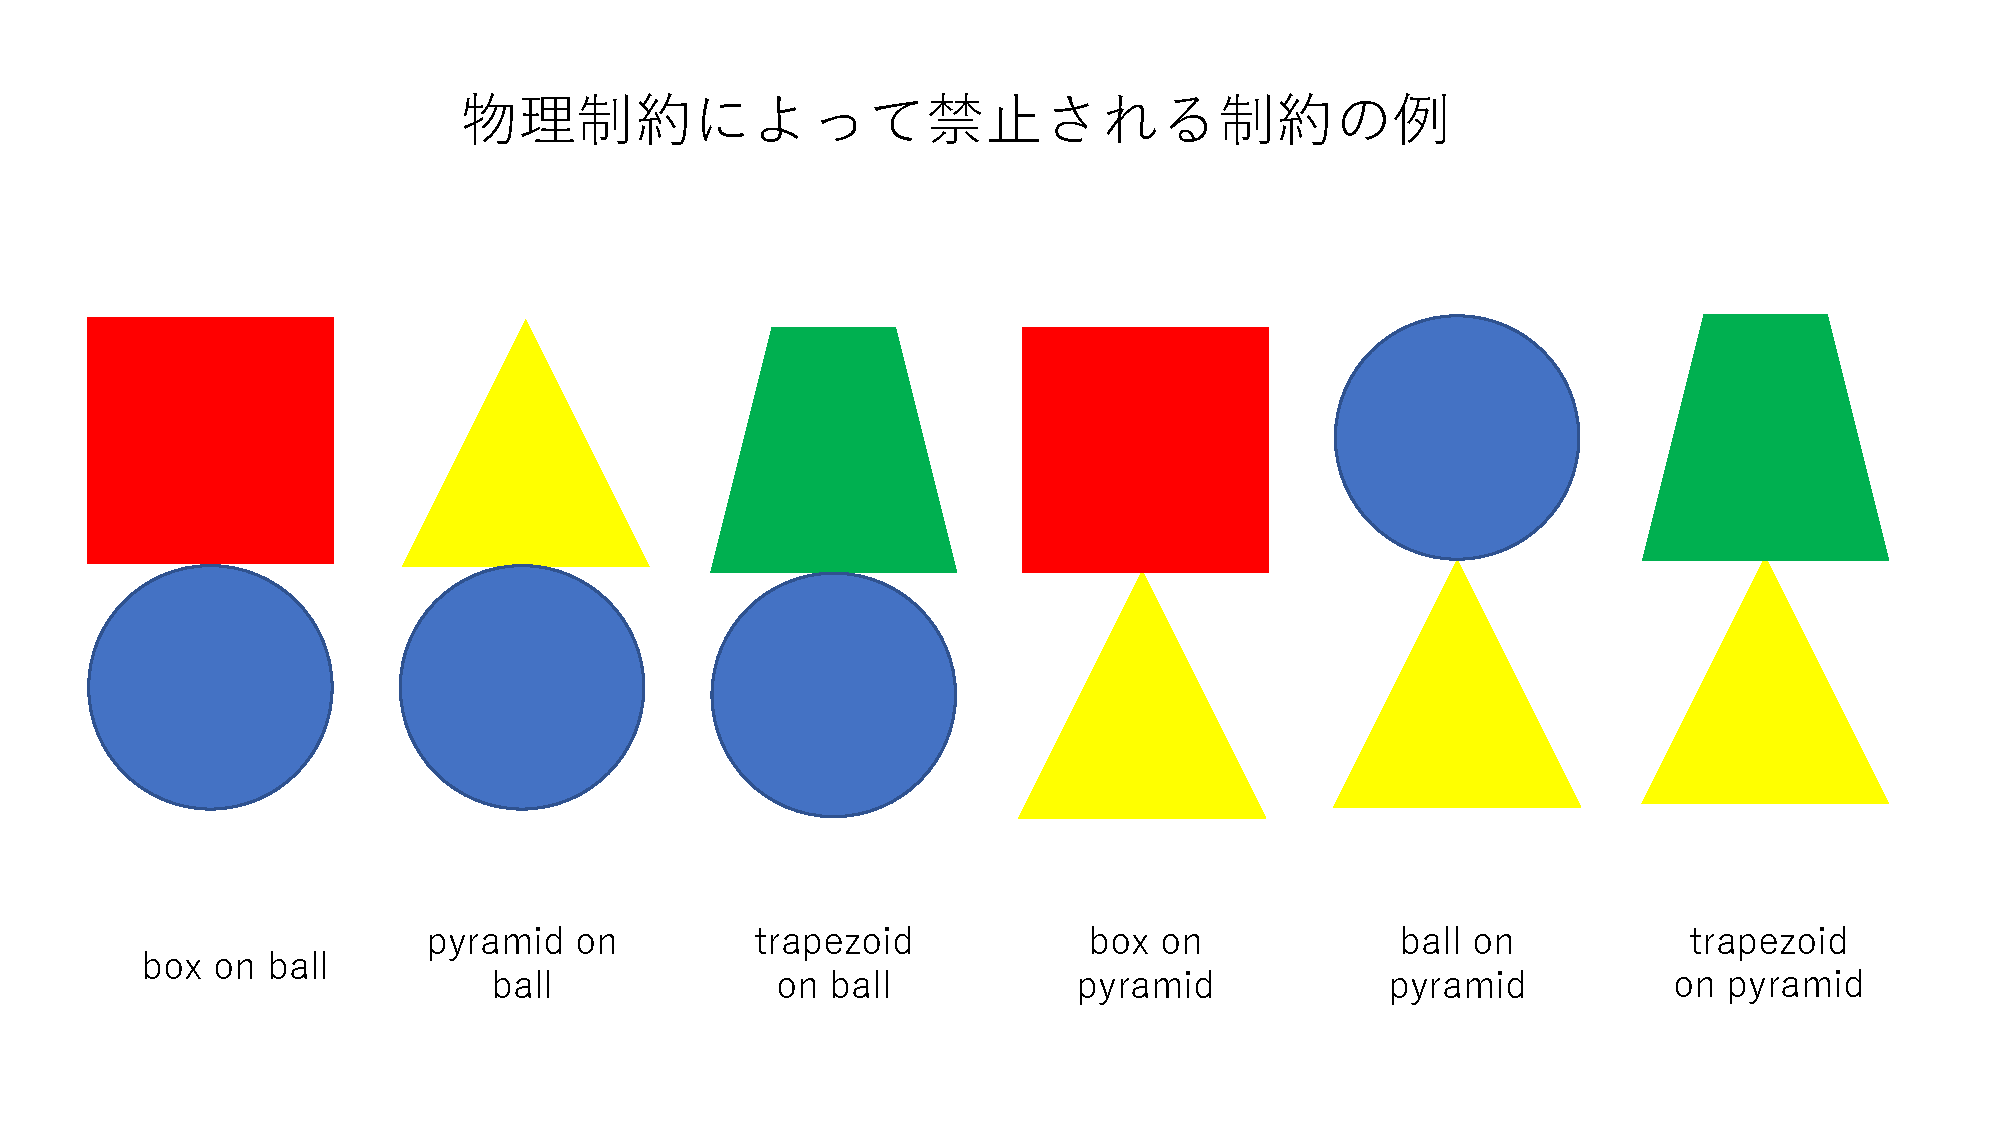
\includegraphics[scale=0.35]{images/prohibit-rules.pdf}
%   \caption{物理制約によって禁止される制約の例}
% \end{figure}

\subsection{実装}
まず,Attributionsクラス内部に,禁止制約への新たなルールの挿入/削除/編集を行う以下のメソッドを追加した.
\begin{description}
\item[insertProhibitRules(ArrayList \textless String\textgreater targetRules)] 新たなルールを挿入するメソッド
\item[deleteProhibitRules(ArrayList \textless String\textgreater targetRules)] 指定したルールを削除するメソッド
\item[editProhibitRules(String beforeRule, String afterRule)] 指定したルールを編集するメソッド
\end{description}
以下に各メソッドについてソースコードと説明を示す.

はじめに,新たなルールを挿入するメソッドを示す.
\begin{lstlisting}[caption=insertProhibitRulesメソッドの実装, label=mid]
    public void insertProhibitRules(ArrayList<String> targetRules) {
		prohibitRules.addAll(targetRules);
		prohibitBlockStates.clear();
		prohibitBlockStates = editStatementList(prohibitRules);
	}
\end{lstlisting}
まず,挿入する対象のルールリストを引数で受け取り,2行目で既存の禁止制約リストに全て加える.
さらに,3行目ではブロック名による禁止制約リストを一度全て削除し,更新されたルールリストを元にして,4行目で作成し直している. \\

次に,指定されたルールを削除するメソッドを示す.
\begin{lstlisting}[caption=deleteProhibitRulesメソッドの実装, label=mid]
    public void deleteProhibitRules(ArrayList<String> targetRules) {
		for(String targetRule: targetRules) {
			prohibitRules.remove(targetRule);
		}
		prohibitBlockStates.clear();
		prohibitBlockStates = editStatementList(prohibitRules);
	}
\end{lstlisting}
まず,削除する対象のルールリストを引数で受け取り,2~4行目で既存の禁止制約リストから削除する処理を行なっている.
5,6行目では先ほど同様にブロック名による表現に反映している. \\

続いて,指定されたルールを編集するメソッドを示す.
\begin{lstlisting}[caption=editProhibitRulesメソッドの実装, label=mid]
    public void editProhibitRules(String beforeRule, String afterRule) {
		prohibitRules.remove(beforeRule);
		prohibitRules.add(afterRule);
		prohibitBlockStates.clear();
		prohibitBlockStates = editStatementList(prohibitRules);
	}
\end{lstlisting}
まず,編集する対象のルールリストを引数で受け取り,2行目で既存の禁止制約リストから編集前ルールを削除し,3行目で編集後ルールを挿入する処理を行なっている.
4,5行目では先ほど同様にブロック名による表現に反映している. \\

また,Presenterクラスにおいてもこれらを利用する同名メソッドを定義した. \\
なお,これらのメソッドでは,引数で受け取るリストの要素数によって,GUIへの反映処理を切り分けられる実装となっている.
具体的には,要素数が0の場合やnullといった場合には,処理を行うことができないように,GUIへとフィードバックを行うように変更した.

\subsection{実行例}
以下に,今回追加したメソッドをテストした結果を示す.
\begin{lstlisting}[caption=editProhibitRulesメソッドの実装, label=mid]
    ~/Programming2/individual_report/attributions
    ●java Test   
    **** Attribution rules ****
    A is blue
    A is ball
    B is green
    B is trapezoid
    C is red
    C is box
    ###### Add prohibitRule ######
    ****** ProhibitRule:ball on ball ******
    ****** ProhibitRule:trapezoid on ball ******
    ****** ProhibitRule:trapezoid on trapezoid ******
    ****** ProhibitRule:box on ball ******
    ****** ProhibitRule:box on box ******
    ****** ProhibitRule:pyramid on ball ******
    ****** ProhibitRule:ball on pyramid ******
    ****** ProhibitRule:box on pyramid ******
    ****** ProhibitRule:trapezoid on pyramid ******
    ****** ProhibitRule:pyramid on pyramid ******
    ++++++ EditStatement ++++++
    ball on ball =====> A on A
    trapezoid on ball =====> B on A
    trapezoid on trapezoid =====> B on B
    box on ball =====> C on A
    box on box =====> C on C
    pyramid on ball =====> pyramid on A
    ball on pyramid =====> A on pyramid
    box on pyramid =====> C on pyramid
    trapezoid on pyramid =====> B on pyramid
    pyramid on pyramid =====> pyramid on pyramid
    
    ----- insert rules -----
    blue on red
    green on blue
    ++++++ EditStatement ++++++
    ball on ball =====> A on A
    trapezoid on ball =====> B on A
    trapezoid on trapezoid =====> B on B
    box on ball =====> C on A
    box on box =====> C on C
    pyramid on ball =====> pyramid on A
    ball on pyramid =====> A on pyramid
    box on pyramid =====> C on pyramid
    trapezoid on pyramid =====> B on pyramid
    pyramid on pyramid =====> pyramid on pyramid
    blue on red =====> A on C
    green on blue =====> B on A
    
    ----- delete rules -----
    blue on red
    ++++++ EditStatement ++++++
    ball on ball =====> A on A
    trapezoid on ball =====> B on A
    trapezoid on trapezoid =====> B on B
    box on ball =====> C on A
    box on box =====> C on C
    pyramid on ball =====> pyramid on A
    ball on pyramid =====> A on pyramid
    box on pyramid =====> C on pyramid
    trapezoid on pyramid =====> B on pyramid
    pyramid on pyramid =====> pyramid on pyramid
    green on blue =====> B on A
    
    変更前のルール:green on blue
    変更後のルール:yellow on blue
    ++++++ EditStatement ++++++
    ball on ball =====> A on A
    trapezoid on ball =====> B on A
    trapezoid on trapezoid =====> B on B
    box on ball =====> C on A
    box on box =====> C on C
    pyramid on ball =====> pyramid on A
    ball on pyramid =====> A on pyramid
    box on pyramid =====> C on pyramid
    trapezoid on pyramid =====> B on pyramid
    pyramid on pyramid =====> pyramid on pyramid
    yellow on blue =====> yellow on A
\end{lstlisting}

3~31行目で属性ルールおよび禁止制約の追加と,禁止制約をブロック名による表現に変換する処理の結果を示している.
ここまでは,前回課題での実装範囲と同じである. \\

33~48行目においては,禁止制約挿入処理とブロック名での表現への変換処理の結果を示している.
特に注目すべきは,47・48行目で,これらは新たに挿入された禁止制約の影響を受けた部分である.
先ほどは存在しなかった
\begin{verbatim}
    blue on red=====>A on C
    green on blue=====>B on A
\end{verbatim}
という表現が現れている. \\

50~63行目においては,禁止制約削除処理とブロック名での表現への変換処理の結果を示している.
特に注目すべきは,62行目と63行目の間で,先ほどは存在した
\begin{verbatim}
    blue on red=====>A on C
\end{verbatim}
が削除されてなくなっている.

65~78行目においては,禁止制約編集処理とブロック名での表現への変換処理の結果を示している.
特に注目すべきは,78行目で,先ほどは
\begin{verbatim}
    green on blue=====>B on A
\end{verbatim}
となっていた部分が,
\begin{verbatim}
    yellow on blue=====>yellow on A
\end{verbatim}
として編集されている.

\subsection{考察}
今回,禁止制約を自由に挿入/削除/編集することができる機能を追加したことによって,
前回課題では物理法則に則ったもののみであったが,ユーザー独自のカスタマイズを行うことが可能となった.
特に,色などの属性による制約を加えることによって,さらに複雑な問題設定が可能となる. \\
プランニングなど,知識ベース型の人工知能システムは,十分な知識を取得可能な場面においては,
データ駆動型のシステムに比べて低コストで高精度の予測を行えることもあり,現在でも非常に有効な手段である.
むしろ,このような場合には,知識ベース型のシステムを選択すべきであり,いたずらにデータ駆動型の機械学習を導入すべきではないとも考えられる. \\
双方の特徴を知り,長所・短所を正しく認識した上で社会への応用が可能となることを胸に刻む必要があると感じた.
また,ただ理論やアルゴリズムを組み上げるのみでは十分ではなく,「多くの人に使ってもらえるようなUI/UX」を考える必要もある.
情報プロダクトにおいても,エンジニアの自己満足ではなくユーザーの側に立ってプロダクトを作ることができて初めて社会的価値があると言える. \\
さらに,本演習前半の「Javaによる知識システム実装」では,知識システムプログラムの改良とGUI実装を行なうことを通して,
グループワークの難しさも体験した.
個人それぞれの事情や性格が違うので,なかなか上手くまとまらない場面もあり,毎回レポートやプログラムの完成が提出期限間際となっていた.
私個人としては,早めに課題を終わらせておく性格であるため,そうでない人と協調して作業を行うことは非常に難しく感じた.
しかし,GUIなど特定の個人が興味を抱いている分野に関しては率先して取り組む姿が見られ,担当者に頼もしさを感じることもあった.
実際に社会に出た際に求められるスキルとして,グループ開発は必須となってくると考えられるので,現段階から少しでもそれを体験できたのは非常に良かったと感じている.


% 参考文献
\begin{thebibliography}{99}
\bibitem{notty} Javaによる知能プログラミング入門 --著:新谷 虎松 \\
\end{thebibliography}

\end{document}